\section{Approach}
\label{sec:approach}

\todo{If it has not yet been mentioned that we're throwing a GNN at the AST, put that here}

\subsection{Graph Construction}


Because ``graph neural nets'' are such a general framework, the inductive bias for the solution comes primarily from how the input graph is constructed.
Specifically, we must decide on the nodes and edges of our generated graph.
We choose to include the full set of nodes in each program's AST as the nodes in the input graph.
This allows us to include all potentially relevant structure: we have not only the source level tokens in the source file, but also the abstract structures that those tokens form.

Graph edges are significantly more complicated.
We want to take advantage of all of the important connections that we know about in the program, while also trying to avoid creating as many useless edges as possible, both to help with computation and to induce a stronger prior over the solutions we think might be valid.
Specifically, we take advantage of our knowledge of the important local and nonlocal interactions between various parts of programs, similar to how convolutional networks assume some strong relationship between local pixels~\cite{henaff2015deep}.
There are three specific priors we bake into the edges in our generated graph:

\paragraph{Nodes near a variable in the AST reflect something about that variable's type.}\
\ % need a space after paragraph
\begin{lstlisting}
  let x = y * 2;
\end{lstlisting}
A human trying to infer the type of the variable \texttt{x} in the above code may decide that since the result of multiplying something by a number is almost always a number, \texttt{x} is probably a number.
This corresponds exactly to two types of edges that we include in our generated graph, an \texttt{AstChild} edge from parents to their child nodes in the AST, and an \texttt{AstParent} edge from children to their parent in the AST.

\par\paragraph{Nodes near a variable in the file reflect something about that variable's type.}
\ % need a space after paragraph
\begin{lstlisting}
  let x = 1;
  let y = x;
  ...
  let x = "foo";
\end{lstlisting}
It is clear that both ordering and locality matter in determining the type of \texttt{y}: in the AST, the two statements assigning to \texttt{x} are equidistant and directionally indistinguishable, but the actual \emph{token stream} of file reflects that the first assignment to \texttt{x} precedes the assignment to \texttt{y}, meaning that it may be more likely to affect the type of \texttt{y}, and is also closer, meaning the two statements are more likely to be related.
Because of this, we include two more types of edges in the induced graph, a \texttt{TokenNext} edge from a token to its neighbor in the source file, and a \texttt{TokenPrev} edge which is the reverse.

\paragraph{Nodes that use or define the same variable give information about each other.}
\ % need a space after paragraph
\begin{lstlisting}
  let x = 1;
  ...
  let y = a + (b + (... + x));
\end{lstlisting}
Although the two statements may be arbitrarily nonlocal in both the AST and the source file, they are clearly related, in that \texttt{x}'s type probably influences \texttt{y}'s type.
Because of this, we include one final types of edge, a \texttt{Variable} edge between any of a variable's use and definition.

\paragraph{Example.}
With all of the above nodes and edges included, we generate (a cleaned up version of) the graph shown in Figure~\ref{fig:ast-graph} for the following problem:
\begin{lstlisting}
  let x := 5;
  x = x + 2;
  console.log(x);
\end{lstlisting}

\begin{figure}
  \centering
  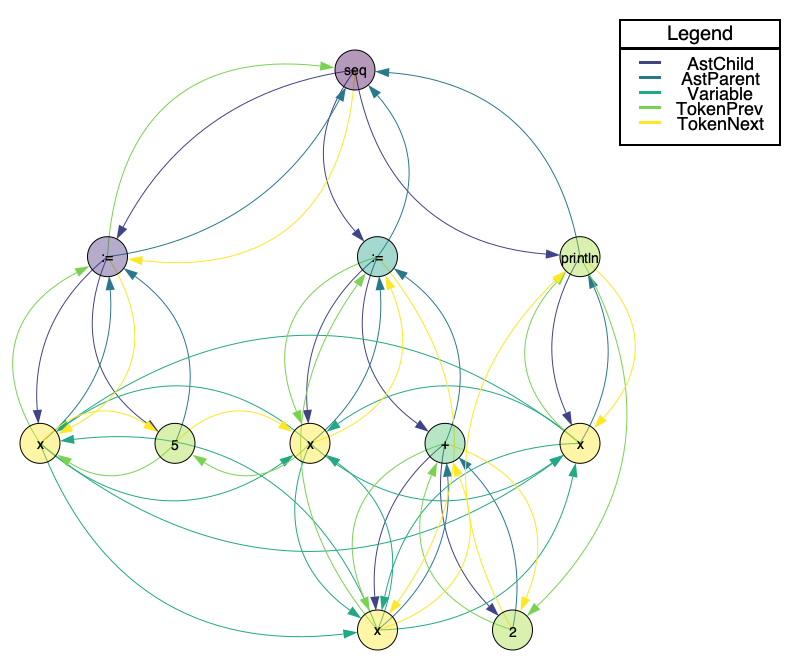
\includegraphics[width=\linewidth]{img/gen_graph}
  \caption{Generated graph for a simple example}
  \label{fig:ast-graph}
\end{figure}

\subsection{Embeddings}

\todo{fill out this section}

\subsection{Architecture}

We implemented our graph neural nets using DeepMind's Graph Nets framework~\cite{deepmind2018graph}.

\subsection{Train Test Split}

\paragraph{Transfer Learning.}
\todo{talk about cool transfer learning stuff here.}

\subsection{Implementation}

We implemented our type prediction algorithm using using DeepMind's Graph Nets framework~\cite{deepmind2018graph}, along with a significant amount of custom TensorFlow~\cite{google2015tensorflow} to collect metrics and perform experiments.


%%% Local Variables:
%%% TeX-master: "main"
%%% End: